\documentclass[tikz,border=12pt]{standalone}
\usepackage[T1]{fontenc}
\usepackage{mathpazo}
\usepackage{amsmath,amssymb}
\usetikzlibrary{arrows.meta, positioning, calc}

\definecolor{stblue}{HTML}{7B97AD}
\definecolor{rwgold}{HTML}{B8995E}
\definecolor{sage}{HTML}{7A9A7E}
\definecolor{dkbrown}{HTML}{3D3530}
\definecolor{wmgray}{HTML}{7B7067}
\definecolor{cream}{HTML}{F9F6F0}
\definecolor{border}{HTML}{D4C9B8}
\definecolor{terracotta}{HTML}{C47A6A}

\begin{document}
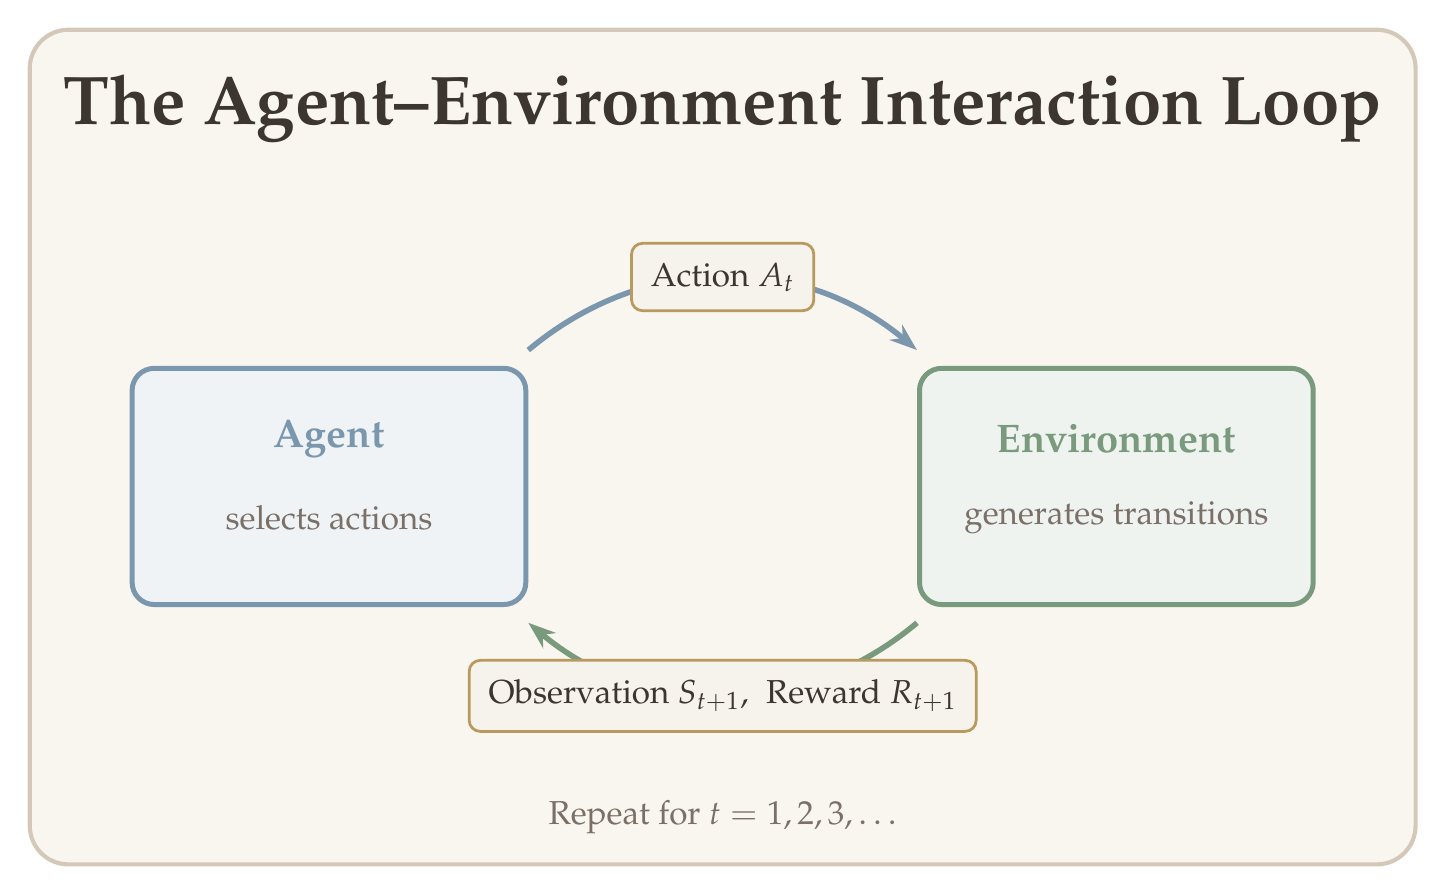
\begin{tikzpicture}[
  >={Stealth[length=3.5mm, width=2.5mm]},
  box/.style 2 args={
    draw=#1, line width=1.8pt, fill=#1!12, rounded corners=8pt,
    minimum width=50mm, minimum height=30mm,
    font=\large, text=dkbrown, align=center, inner sep=6pt},
  lbl/.style={fill=rwgold!12, draw=rwgold, line width=1pt,
    rounded corners=4pt, inner sep=7pt, outer sep=4pt,
    font=\large, text=dkbrown},
]

% Background canvas
\fill[cream, rounded corners=14pt] (-0.8,-4.8) rectangle (16.8,5.8);
\draw[border, rounded corners=14pt, line width=1.5pt] (-0.8,-4.8) rectangle (16.8,5.8);

% Title
\node[font=\Huge\bfseries, text=dkbrown] at (8.0,4.8)
  {The Agent--Environment Interaction Loop};

% === Agent box (left, stblue) ===
\node[box={stblue}{}] (agent) at (3.0,0) {};
\node[font=\Large\bfseries, text=stblue] at (3.0,0.6) {Agent};
\node[font=\large, text=wmgray] at (3.0,-0.4) {selects actions};

% === Environment box (right, sage) ===
\node[box={sage}{}] (env) at (13.0,0) {};
\node[font=\Large\bfseries, text=sage] at (13.0,0.6) {Environment};
\node[font=\large, text=wmgray] at (13.0,-0.4) {generates transitions};

% ============================================================
% TOP ARC: Agent -> Environment  (action)
% Single smooth arc; opaque label node covers the line at midpoint
% ============================================================
\draw[->, line width=2pt, stblue]
  ([yshift=2mm]agent.north east)
  to[out=40, in=140]
  node[pos=0.5, lbl] {Action $A_t$}
  ([yshift=2mm]env.north west);

% ============================================================
% BOTTOM ARC: Environment -> Agent  (observation, reward)
% Single smooth arc; opaque label node covers the line at midpoint
% ============================================================
\draw[->, line width=2pt, sage]
  ([yshift=-2mm]env.south west)
  to[out=220, in=320]
  node[pos=0.5, lbl] {Observation $S_{t+1}$,\; Reward $R_{t+1}$}
  ([yshift=-2mm]agent.south east);

% === Bottom annotation ===
\node[font=\large, text=wmgray] at (8.0,-4.2)
  {Repeat for $t = 1, 2, 3, \ldots$};

\end{tikzpicture}
\end{document}
